\documentclass[12pt]{article}
\usepackage[utf8]{inputenc}
\usepackage{lipsum}
\usepackage{pifont}
\usepackage{outlines}
\usepackage{multirow}
\usepackage{subcaption}
\usepackage{adjustbox}
\usepackage{amsmath}
\usepackage{makecell}
\usepackage{fancyhdr}
\usepackage{float}
\usepackage{graphicx}
\usepackage{tikz,xcolor}
\usepackage{karnaugh-map}
\usepackage{longtable}
\usepackage[a4paper, total={7in, 10in}]
{geometry}

\usepackage[skip =10pt, indent =0pt]{parskip}

\pagestyle{fancy}
\fancyhead[C]{Computer Architecture Sessional Assignment 1}
\fancyhead[R]{}
\fancyhead[L]{CSE 306}
\fancyfoot[R]{Prepared using \LaTeX}

\title{CSE 306 OFFLINE 1 LABORATORY REPORT}
\author{\textsuperscript{1}Sadia Tabassum, \textsuperscript{2}Alina Zaman, \textsuperscript{3}Md.Shafiul Haque ,\\\textsuperscript{4}Mayesha Rashid, \textsuperscript{5}Saha Kuljit Shantanu}
\date{20 December 2022}





\begin{document}

\maketitle

\section{Introduction}
An \textit{Arithmetic Logic Unit} (ALU) is a multi-operation, combinational-logic digital function. It can perform a set of basic arithmetic and logical operations. The ALU has a number of selection lines to select a particular operation in the unit. The selection lines are decoded or multiplexed
within the ALU so that k selection variables can specify up to 2\textsuperscript{k} distinct operations.\\

In this experiment, three selection variables (cs2, cs1, cs0) have been used which can enable to perform 2\textsuperscript{3} = 8 distinct operations. The four data bit inputs from A are combined with the four bit inputs from B to generate an operation at the outputs. \\

In our ALU design, we use a 4-bit status register. This status register contains 4 status bits that are denoted by C(Carry), S(Sign), V(Overflow) and Z(Zero). These status bits change during arithmetic operations. They indicate the following changes:
\begin{itemize}
    \item[\ding{227}] \textbf{CF:} Carry Bit C is set 1 when the output carry of the 4 Bit Parallel Adder in ALU(IC 7483 used in this experiment) is 1. If carry output is not obtained, it is set to 0 by default.
    \item[\ding{227}] \textbf{SF:} Sign Bit S is set 1 when the most significant bit of the output of the ALU is 1, it is set 0 when the most significant bit is 0. 
    \item[\ding{227}] \textbf{OF:} Overflow Bit V is set 1 if the X-OR of carries C4 and C5 is 1 (which indicates overflow), otherwise it is set 0. Overflow occurs when two same signed numbers are added and the sign bit of the output is different.
    \item[\ding{227}] \textbf{ZF:} Zero Bit Z is set 1 if the output is zero, otherwise the Z bit is set 0.
\end{itemize}


\section{Problem Specification with Assigned Instruction}

Depending on the selection bits cs2, cs1 and cs0, the design of two four bit operands A and B are supposed to operate according to the following table where some arithmetic or logical operations are defined to perform that correspond to the combination of the control signals.

%\renewcommand{\arraystretch}{2}
\large{
\begin{table}[H]

    \centering
    \begin{adjustbox}{width = \textwidth}
    
    \begin{tabular}{|c c c|c|c|}
    \hline
    CS2 & CS1 & CS0 & Functions & Expected Equation\\

    \hline

    X & 0 & 0 & Subtraction with borrow & A + $\bar{B}$\\

    0 & 0 & 1 & Transfer A & A\\

    X & 1 & 0 & XOR & A $\oplus$ B\\

    0 & 1 & 1 & NEG A & $\bar{A}$ + 1\\

    1 & 0 & 1 & OR & A $\cup$ B\\

    1 & 1 & 1 & Subtraction & A + $\bar{B}$ + 1\\

    \hline
    
    \end{tabular}
    
    
    \end{adjustbox}
    \caption{Table For Specified Instructions}
    \label{tab:Instructiontable}
\end{table} 
}
%\renewcommand{\arraystretch}{1}

\section{Detailed Design Steps with k-maps}

\subsection{Designing}
From the table \ref{tab:Instructiontable} three variables can be defined for addition purpose while preparing the ALU.\\

Variable \textit{X} will be a four bit representation of A ( A or $\bar{A}$ ) or any logical operation of A with B ( AND OR XOR). \\

Variable \textit{Y} will be a four bit representation of B ( B or $\bar{B}$ )\\

Variable \textit{Z} will be the Carry input to the adder, which is 1 bit (Either 0 or 1) \\

The table will now be designed with the three control Signals CS2,CS1,CS0 as input and \textit{X},\textit{Y} and \textit{Z} as output. where \textit{X},\textit{Y} and \textit{Z} are functions of A or B.\\

\subsection{Table of Inputs and Outputs}


\begin{table}[H]

    \centering
    \begin{adjustbox}{width =.6 \textwidth}
    
    \begin{tabular}{|c c c|c|c|c|}
    \hline
    CS2 & CS1 & CS0 & \textit{X} & \textit{Y} & \textit{Z}\\

    \hline

    0 & 0 & 0 & A & $\bar{B}$ & 0\\

    0 & 0 & 1 & A & 0 & 0\\

    0 & 1 & 0 & A $\oplus$ B & 0 & 0\\

    0 & 1 & 1 & $\bar{A}$ & 0 & 1\\

    1 & 0 & 0 & A & $\bar{B}$ & 0\\
    
    1 & 0 & 1 & A $\cup$ B & 0 & 0\\

    1 & 1 & 0 & A $\oplus$ B & 0 & 0\\
    
    1 & 1 & 1 & A & $\bar{B}$ & 1\\

    \hline
    
    \end{tabular}
    
    \end{adjustbox}
    \caption{Table For Output Function}
    \label{tab:IOtable}
\end{table} 

%\renewcommand{\arraystretch}{1}

\subsection{Forming Equations for \textit{X}}

The equation of \textit{X} was obtained by the 4*1 Multiplexer (IC 74LS153). As the output was four bit and the IC was a dual Mux, hence two IC's were required for the generation of four bit \textit{X}.\\

Based on the output function \textit{X} obtained from the table \ref{tab:IOtable}, the Multiplexer Equations can be implemented. The concept we used here are:

\begin{itemize}
    \item[\ding{228}]{CS1 and CS0 were used as selector bits }
    \item[\ding{228}]{\textit{X\textsubscript{i}} is a function of CS2,A\textsubscript{i},B\textsubscript{i}, where i = 4,3,2,1}
\end{itemize}

\renewcommand{\arraystretch}{1}

\begin{table}[H]

    \centering
    \begin{adjustbox}{width =.6 \textwidth}
    
    \begin{tabular}{|c c|c|}
    \hline
    CS1 & CS0 & \textit{X\textsubscript{i}}(CS2,A\textsubscript{i},B\textsubscript{i})\\

    \hline

    0 & 0 & A\textsubscript{i}\\

    0 & 1 & A\textsubscript{i} $\cup$ B\textsubscript{i} CS2\\

    1 & 0 & A\textsubscript{i} $\oplus$ B\textsubscript{i}\\

    1 & 1 & $\overline{A\textsubscript{i} \oplus CS2}$\\

    \hline
    
    \end{tabular}
    
    \end{adjustbox}
    \caption{Table For Generation of every bit of \textit{X}}
    \label{tab:Xtable}
\end{table} 

\renewcommand{\arraystretch}{1}

\subsection{Forming Equations for \textit{Y}}

\subsubsection{Equation For \textit{Y}}


The equation of \textit{Y} was obtained by the 8*3 Decoder (IC 74LS138). This decoder is active low, operated by two active high enabler and one active low enabler. Only one decoder was sufficient for this task.\\

An equation of \textit{Y} can be generated from the table \ref{tab:IOtable}\\

Using the \textit{SOP} (Sum of Product) System, \textit{Y} has the given equation:

\begin{equation}
    \boldmath Y_i = ( \bar{cs2}\bar{cs1}\bar{cs0} + cs2\bar{cs1}\bar{cs0} + cs2cs1cs0 )\bar{B_i}
    \undoboldmath
    \label{eq0}
\end{equation}

The equation \ref{eq0} may also be reduced to a fundamental version of the equation.But that is not the objective. In order to reduce the number of IC's using the decoder is a better idea.\\

Using the decoder the equation \ref{eq0} can be replaced in the following manner:\\

\begin{equation}
   \boldmath Y_i = \overline{(D_0 D_4 D_7)}. \overline{B_i}
  \undoboldmath
    \label{eq1}
\end{equation}

Hence the equation \ref{eq1} can be more efficient while IC level design and IC usage efficiency is considered.\\

\subsubsection{Table For \textit{Y}}

The table for output function \textit{Y} :


\begin{table}[H]

    \centering
    \begin{adjustbox}{width = .6\textwidth}
    
    \begin{tabular}{|c c c|c|c|}
    \hline
    CS2 & CS1 & CS0 & D & \textit{Y} \\

    \hline

    0 & 0 & 0 & 01111111 & $\bar{B}$\\

    0 & 0 & 1 & 10111111 & 0 \\

    0 & 1 & 0 & 11011111 & 0\\

    0 & 1 & 1 & 11101111 & 0 \\

    1 & 0 & 0 & 11110111 & $\bar{B}$ \\
    
    1 & 0 & 1 & 11111011 & 0\\

    1 & 1 & 0 & 11111101 & 0\\
    
    1 & 1 & 1 & 11111110 & $\bar{B}$ \\

    \hline
    
    \end{tabular}
    
    \end{adjustbox}
    \caption{Table For Output Function}
    \label{tab:IOtable}
\end{table} 

\renewcommand{\arraystretch}{1}

\subsection{Forming Equations of Carry (\textit{Z}) With K-map}

\subsubsection{K-Map For \textit{Z}}


\begin{karnaugh-map}[4][2][1][$cs1cs0$][$cs2$]
    
    \minterms{3,7}
    \maxterms{0,1,2,4,5,6}
    \implicant{3}{7}
    \label{k0}
    
\end{karnaugh-map}

\subsubsection{Equation For \textit{Z}}

From the Karnaugh-map \ref{k0}, the equation of \textit{Z} can be obtained.
\begin{equation}
    \boldmath Z = cs1cs0
    \label{eq2}
\end{equation}

\subsection{Flag Implementation}

\begin{itemize}


\item[\ding{228}] {\textbf{Zero Flag:} Logical OR is done of all 4 bits of the output. Then the OR output is sent to a NOT gate and the output of the NOT gate is the Zero Flag. When the 4 bit output is 0000, zero flag will be 1, otherwise zero flag will be 0.}

\item[\ding{228}] {\textbf{Sign Flag:} Most significant bit of the output is the sign flag. That is, if MSB is 0, sign flag will be 0, otherwise sign flag will be 1.}

\item[\ding{228}] {\textbf{Carry Flag:} Carry flag is the Cout bit of the adder. As it indicates unsigned overflow, if the Cout is 1, that means unsigned overflow has occured, otherwise Carry flag is 0.}

\item[\ding{228}] {\textbf{Overflow Flag:} Overflow flag indicates signed overflow. If two positive numbers are added and the sign bit of the output is 1, or if two negative numbers are added and the sign bit of the output is 0, then overflow has occurred. To identify this, we do XOR of MSB of X, MSB of Y, MSB of output and Cout. Then if odd number of 1's are found, then Overflow flag is 1, otherwise 0.}

\end{itemize}

\subsection{Hardware requirements}

\begin{itemize}
    \item [\ding{228}]{Breadboard}
    \item [\ding{228}]{Breadboard power}
    \item [\ding{228}]{Switches}
    \item [\ding{228}]{Jumper wires}
    \item [\ding{228}]{Professional wires}
    \item [\ding{228}]{Integrated Circuits}
    \begin{outline}[enumerate]
        \1 NOT(7404)
        \1 AND(7408)
        \1 OR(7432)
        \1 ADDER(7483)
        \1 XOR(7486)
        \1 DECODER(74138)
        \1 MULTIPLEXER(74153)
    \end{outline}
    \item [\ding{228}]{Light Emitting Diodes}
    \item [\ding{228}]{9V Power Adapters}
\end{itemize}


%...
\begin{figure}[H]
  \centering
  \begin{subfigure}[b]{0.3\linewidth}
    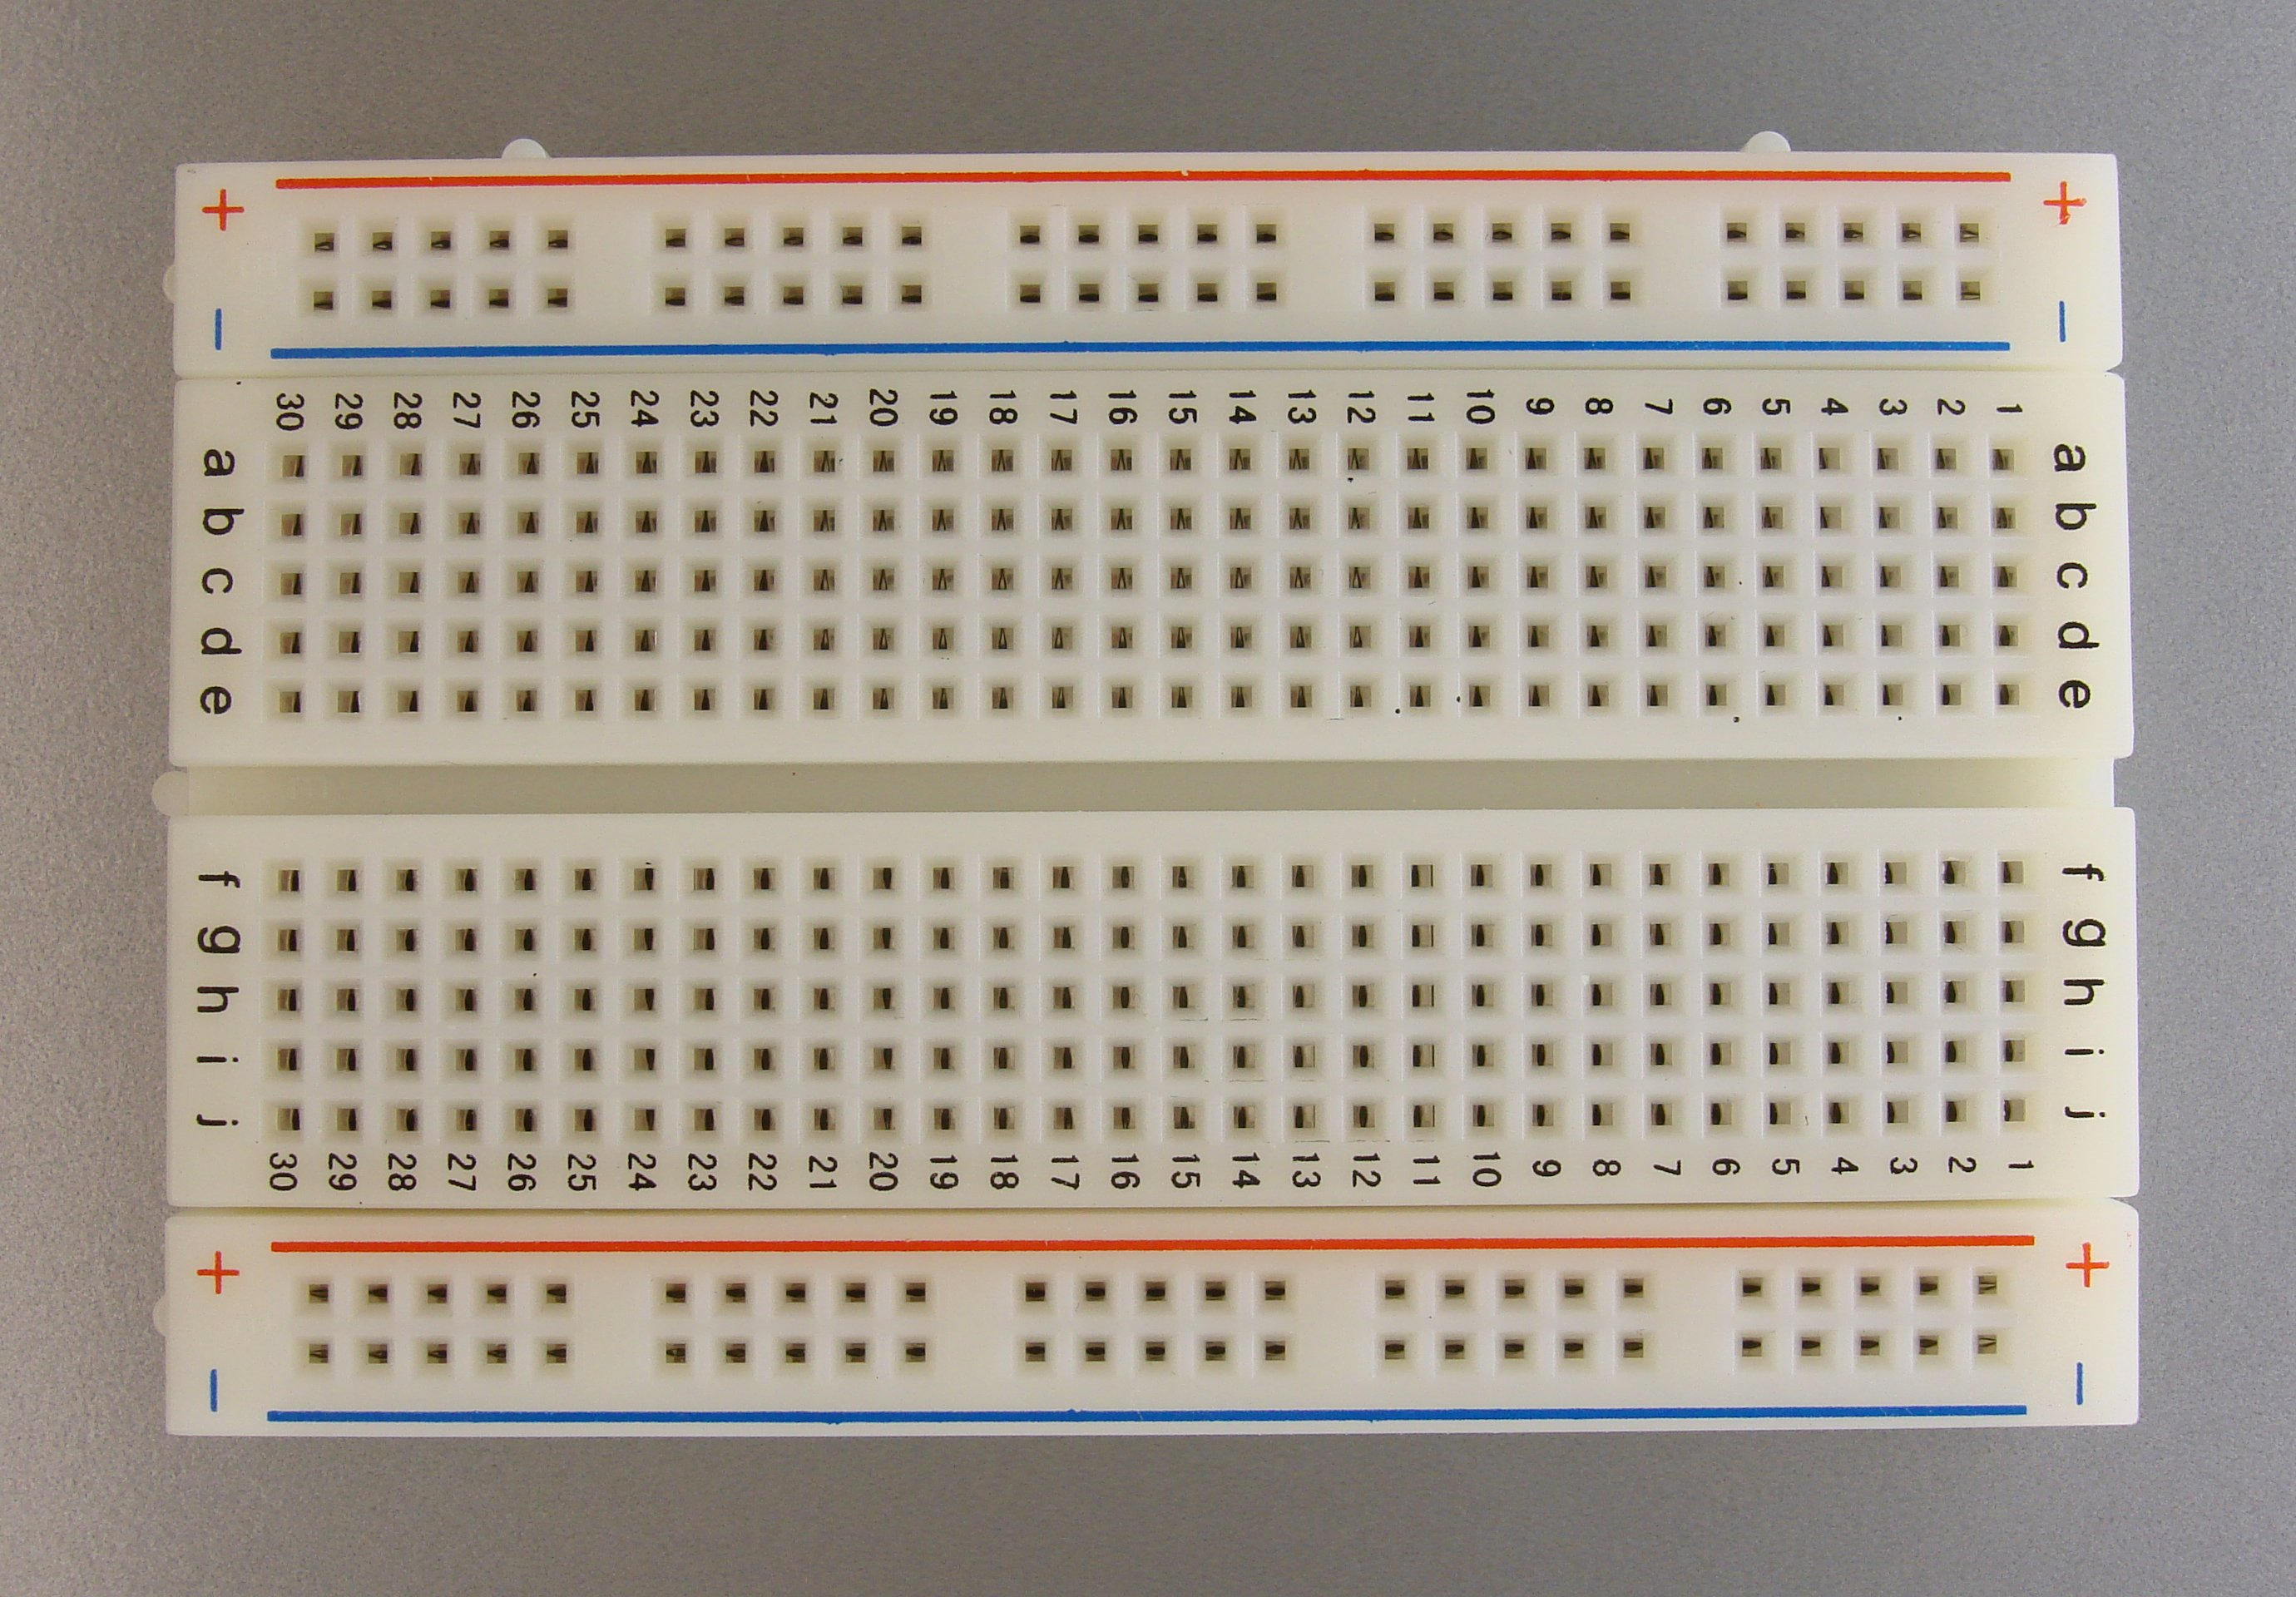
\includegraphics[width=\linewidth]{Breadboard.jpg}
     \caption{Breadboard.}
  \end{subfigure}
  \begin{subfigure}[b]{0.3\linewidth}
    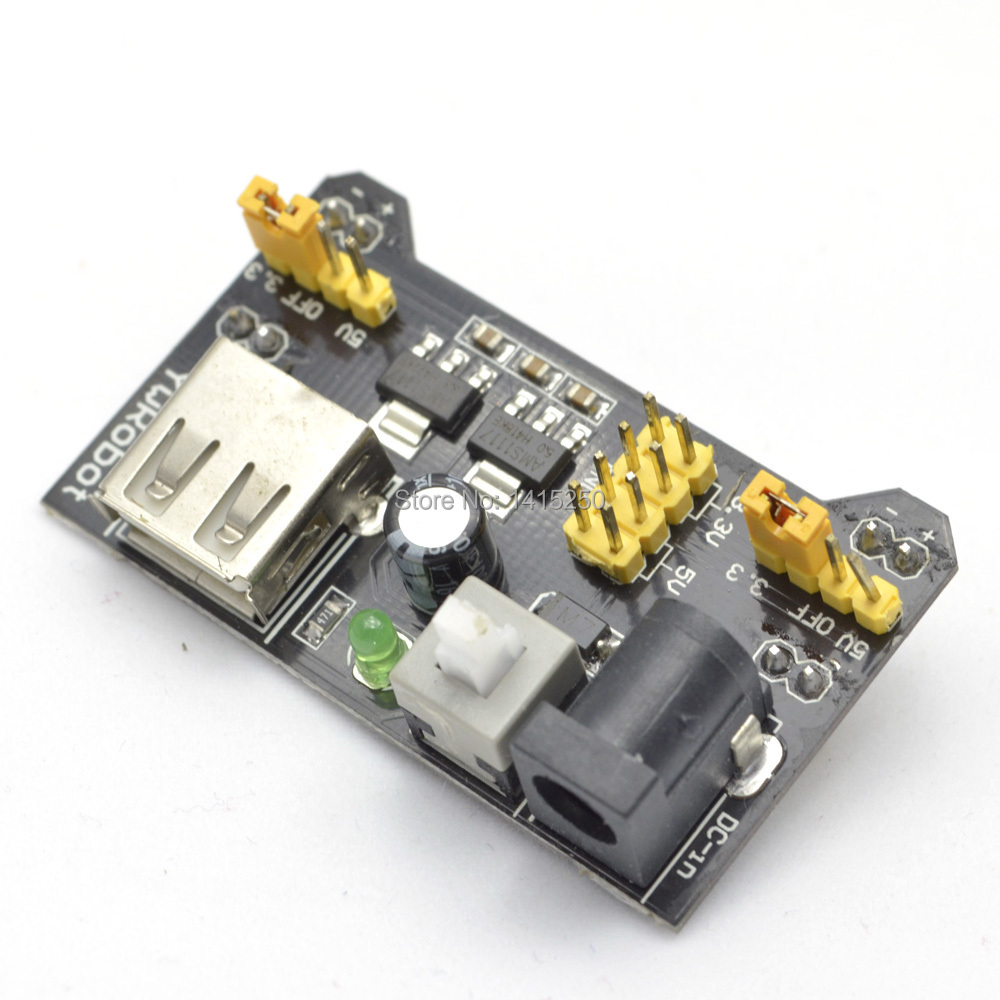
\includegraphics[width=\linewidth]{Breadboard_power.jpg}
    \caption{Breadboard power.}
  \end{subfigure}
  \begin{subfigure}[b]{0.3\linewidth}
    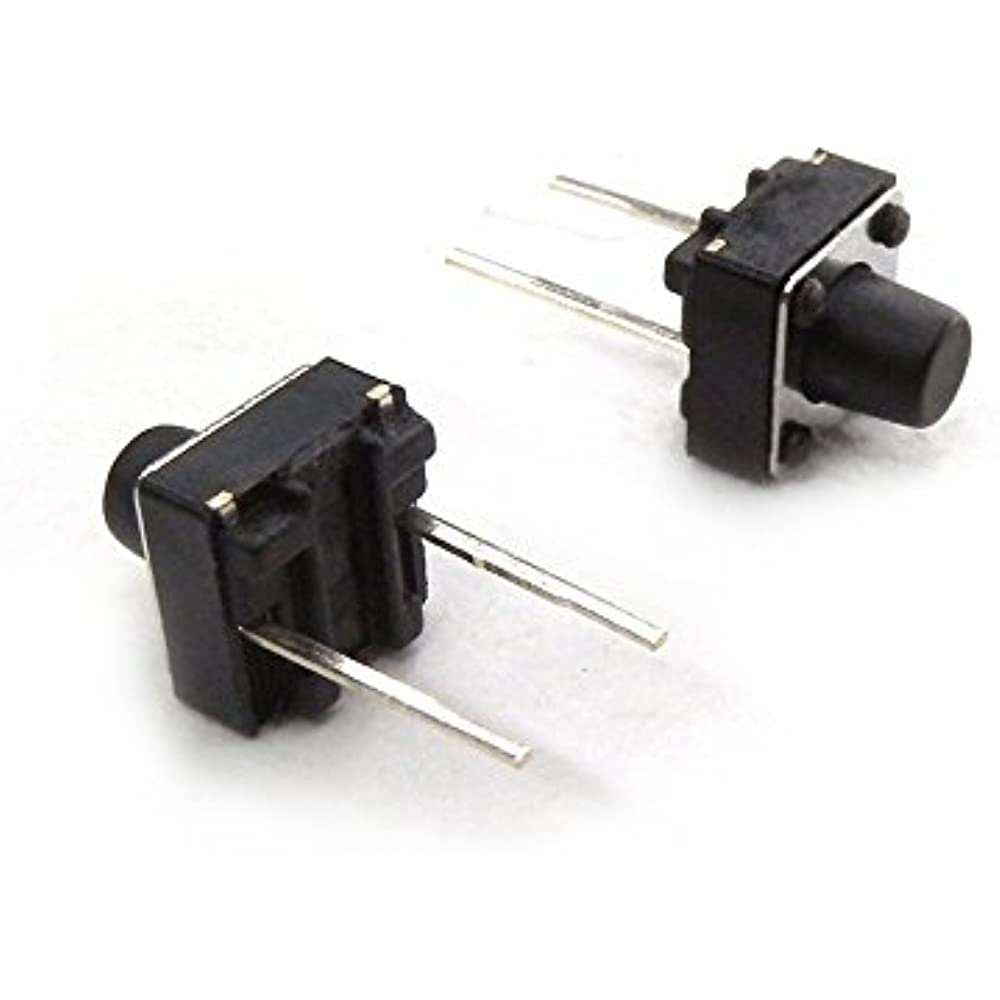
\includegraphics[width=\linewidth]{switch.jpg}
    \caption{Switches.}
  \end{subfigure}
  \begin{subfigure}[b]{0.3\linewidth}
    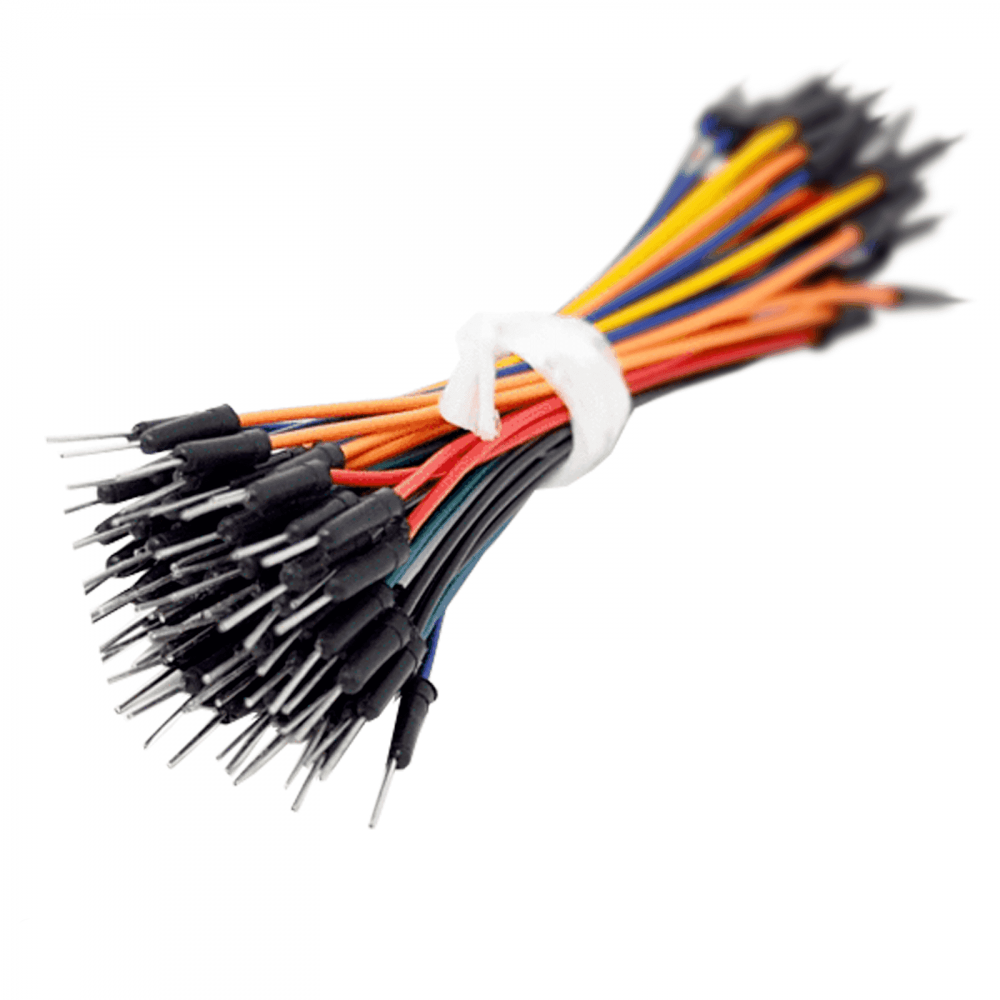
\includegraphics[width=\linewidth]{Wires.png}
    \caption{Jumper wires.}
  \end{subfigure}
  \begin{subfigure}[b]{0.3\linewidth}
    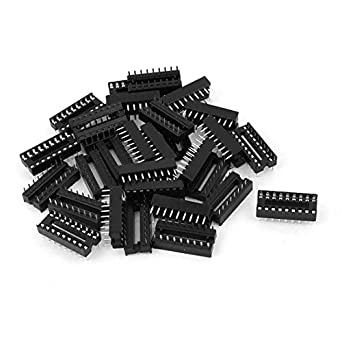
\includegraphics[width=\linewidth]{ICset.jpg}
    \caption{IC set.}
  \end{subfigure}
  \begin{subfigure}[b]{0.3\linewidth}
    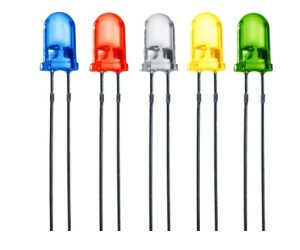
\includegraphics[width=\linewidth]{LED.jpg}
    \caption{LED.}
  \end{subfigure}
  \caption{Hardware requirements.}
  \label{fig:coffee3}
\end{figure}
%...

\section{Truth Table}

For this ALU there are 3 bits for control (cs2,cs1,cs0) and 2$\ding{54}$4 = 8 bits as input. so there are in total 2\textsuperscript{11} = 2048 possible inputs for this ALU. A few  of those is presented in the following table.


\begin{table}[H]

    \centering
    \begin{adjustbox}{width = \textwidth}
    
    \begin{tabular}{|c c c|c|c|c|c|c|c|c|}
    \hline
    CS2 & CS1 & CS0 & A & B & OUTPUT & ZF & CF & SF & OF\\

    \hline

    0 & 0 & 0 & 0000 & 0000 & 1111 & 0 & 0 & 1 & 0\\

    .. & .. & .. & ...  & ...& ...& ...& ...& ...& ...\\

    0 & 0 & 0 & 0001 & 1100 & 0100 & 0& 0& 0& 0\\

    .. & .. & .. & ...  & ...& ...& ...& ...& ...& ...\\

    0 & 0 & 1 & 1000& 0100& 1000& 0& 0& 1& 0\\

    .. & .. & .. & ...  & ...& ...& ...& ...& ...& ...\\

    0 & 0 & 1 & 1101& 0101& 1101& 0& 0 & 1& 0\\

    .. & .. & .. & ...  & ...& ...& ...& ...& ...& ...\\

    0 & 1 & 0 & 0111& 1100& 1011& 0& 0& 1& 0 \\

    .. & .. & .. & ...  & ...& ...& ...& ...& ...& ...\\

    0 & 1 & 0 & 1001& 1000& 0001& 0& 0& 0& 0\\

    .. & .. & .. & ...  & ...& ...& ...& ...& ...& ...\\

    0 & 1 & 1 & 0100& 0010& 1100& 0& 0& 1& 0\\

    .. & .. & .. & ...  & ...& ...& ...& ...& ...& ...\\

    0 & 1 & 1 & 1011& 0110& 0101& 0& 0& 0& 0\\

    .. & .. & .. & ...  & ...& ...& ...& ...& ...& ...\\

    1 & 0 & 0 & 0011& 1101& 0101& 0& 0& 0& 0\\

    .. & .. & .. & ...  & ...& ...& ...& ...& ...& ...\\

    1 & 0 & 0 & 0100& 0011& 0000&1 &1 &0 &0 \\

    .. & .. & .. & ...  & ...& ...& ...& ...& ...& ...\\

    1 & 0 & 1 &0110 & 1100& 1110& 0& 0& 1& 0\\

    .. & .. & .. & ...  & ...& ...& ...& ...& ...& ...\\

    1 & 0 & 1 & 1001& 1101& 1101& 0& 0& 1&0 \\

    .. & .. & .. & ...  & ...& ...& ...& ...& ...& ...\\

    1 & 1 & 0 & 1011& 1100& 0111& 0& 0&0 &0 \\

    .. & .. & .. & ...  & ...& ...& ...& ...& ...& ...\\

    1 & 1 & 0 & 1100& 1100& 0000& 1& 0& 0& 0\\

    .. & .. & .. & ...  & ...& ...& ...& ...& ...& ...\\

    1 & 1 & 1 & 0110& 1001& 1101& 0& 0& 1& 1\\

    .. & .. & .. & ...  & ...& ...& ...& ...& ...& ...\\

    1 & 1 & 1 & 1111 & 1111 & 0000& 1& 1& 0& 0\\

    \hline
    
    \end{tabular}
    
    \end{adjustbox}
    \caption{Table For Specified Instructions}
    \label{tab:Instructiontable}
\end{table} 


\renewcommand{\arraystretch}{1}


\section{Block Diagram}
\begin{center}
    % \centering
    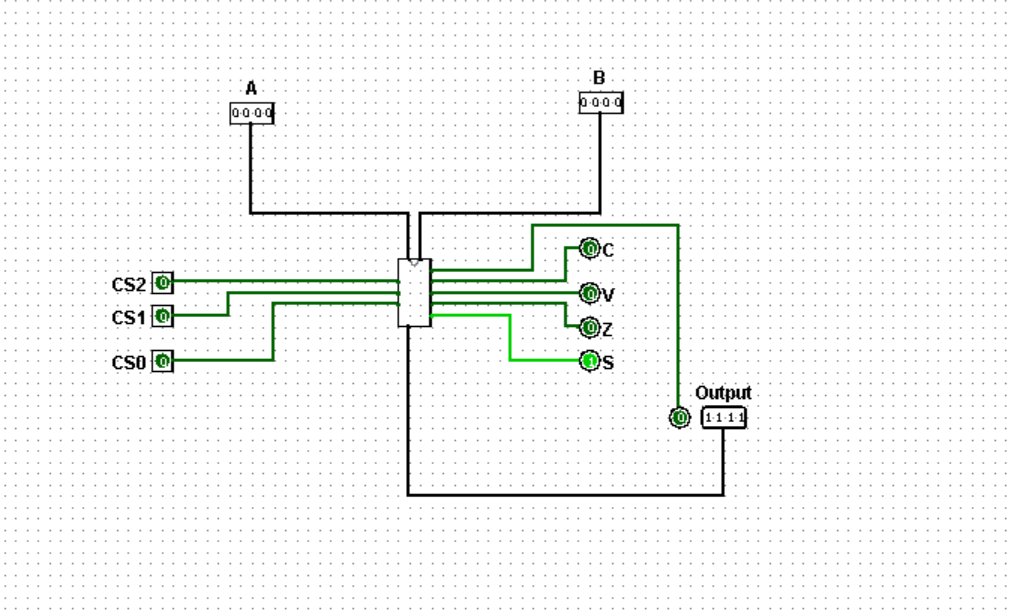
\includegraphics[width=1\textwidth]{block_diagram.png}
    \caption{Block diagram}
    \label{fig:my_label}
\end{center}


\section{Complete Circuit Diagram}

\subsection{ Subcircuit for determination of X}
\begin{center}
    % \centering
    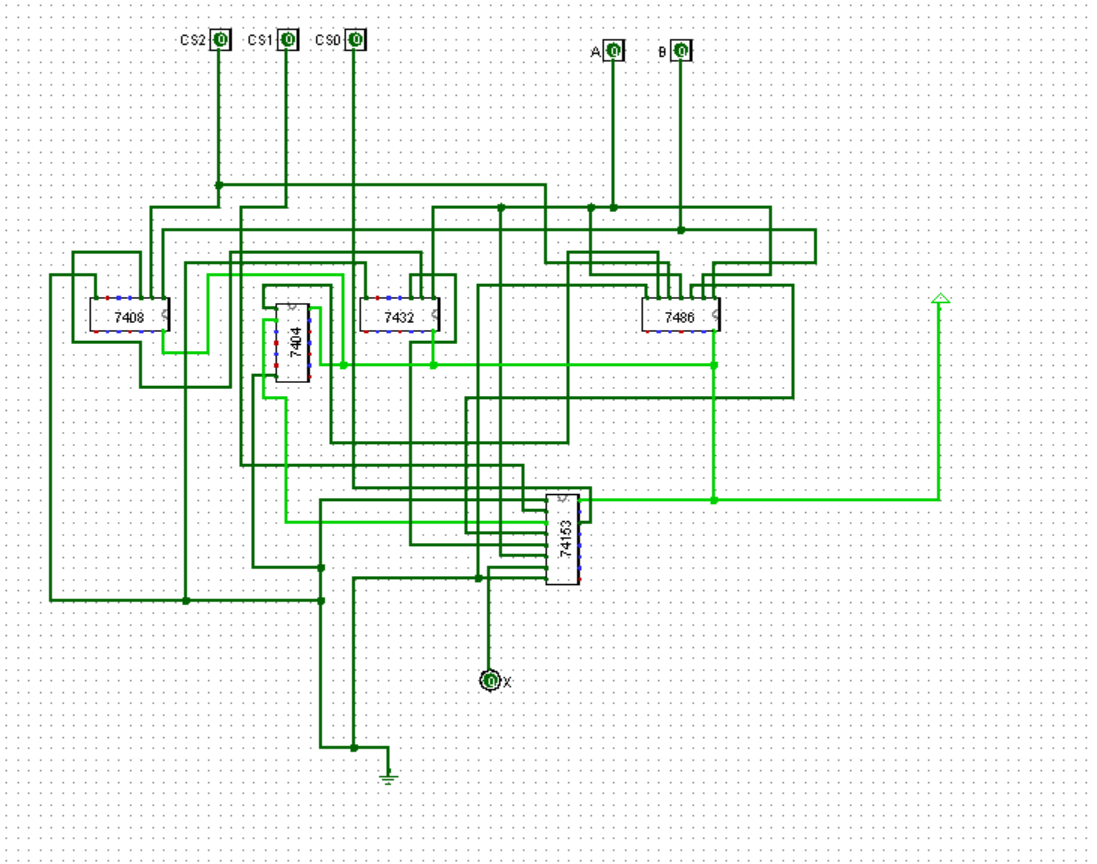
\includegraphics[width=.7\textwidth]{sub_circuit_x.png}
    %\caption{figure 2: Subcircuit for X}
    \label{fig:my_label}
\end{center}

\subsection{Subcircuit for determination of Y \& Z }
\begin{center}
    % \centering
    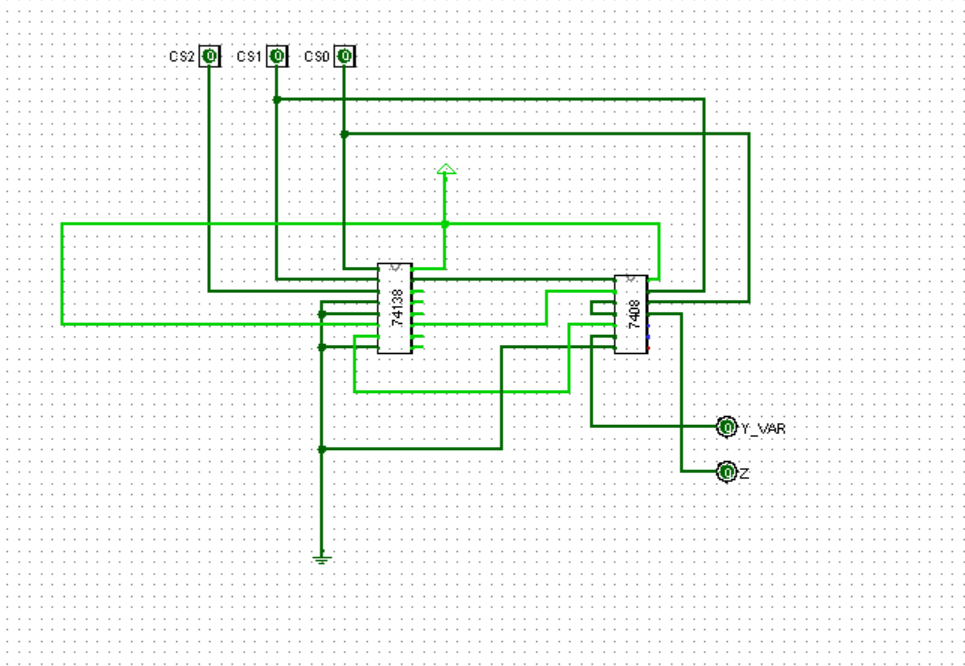
\includegraphics[width=.8\textwidth]{sub_circuit_y_z.png}
    %\caption{figure 2: Subcircuit for X}
    \label{fig:my_label}
\end{center}

\subsection{Designing 4 bit X, Y with Z }
\begin{center}
    % \centering
    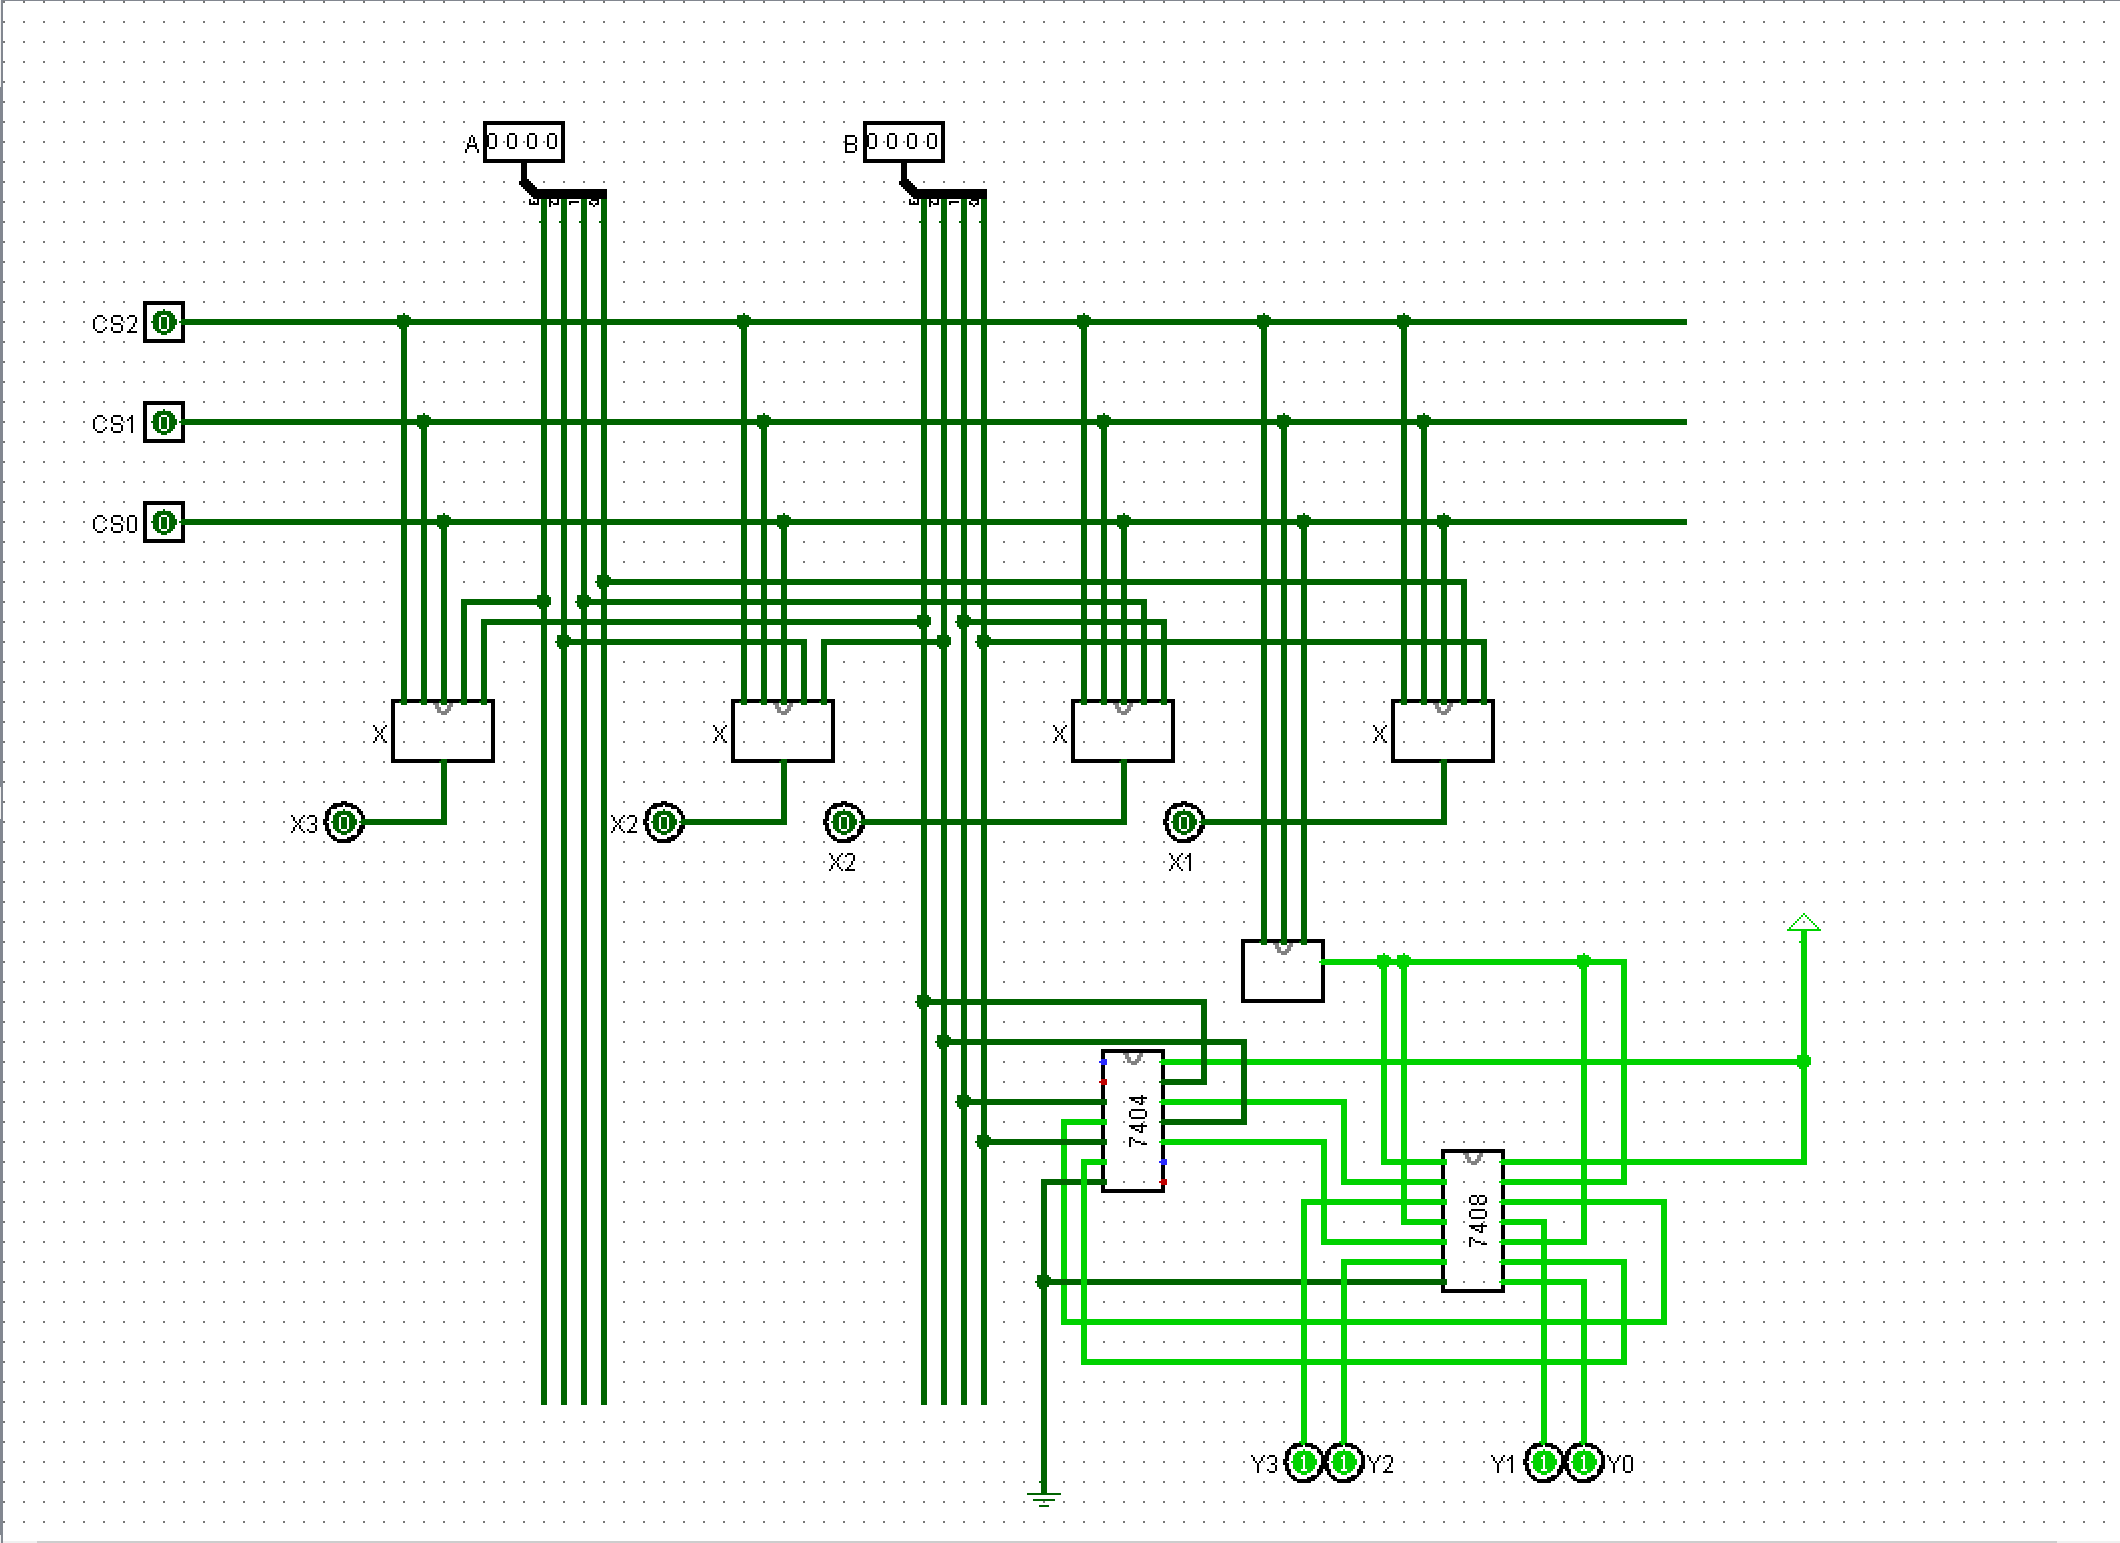
\includegraphics[width=.8\textwidth]{4bit.png}
    %\caption{figure 2: Subcircuit for X}
    \label{fig:my_label}
\end{center}

\subsection{ Subcircuit for the determination of flags}
\begin{center}
    % \centering
    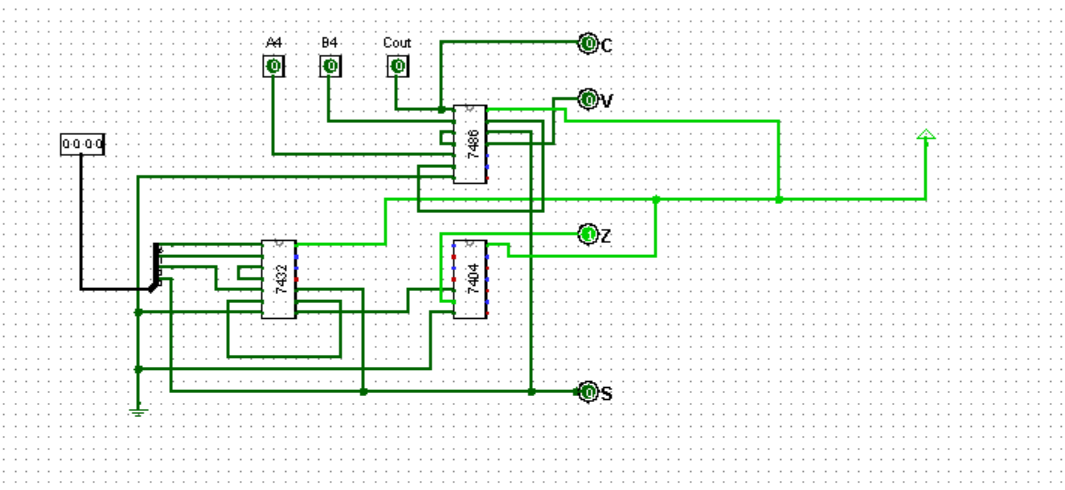
\includegraphics[width=.8\textwidth]{subcircuit_flag.png}
    %\caption{figure 2: Subcircuit for X}
    \label{fig:my_label}
\end{center}

\subsection{ Final circuit diagram with input and output}
\begin{center}
    % \centering
    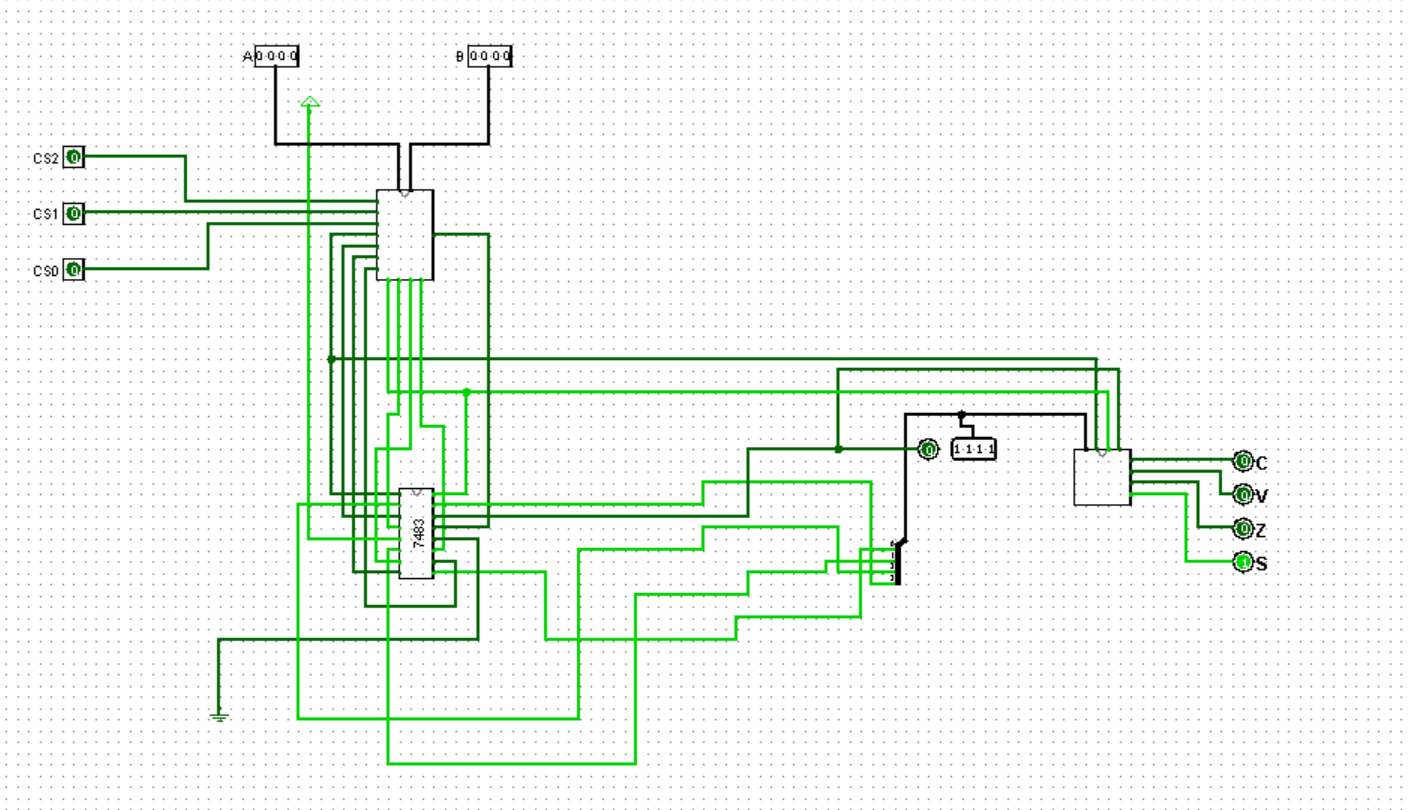
\includegraphics[width=1\textwidth]{final_circuit.png}
    %\caption{figure 2: Subcircuit for X}
    \label{fig:my_label}
\end{center}


\section{ICs used with count as a chart}

\renewcommand{\arraystretch}{2}
\large{
\begin{table}[H]

    \centering
    \begin{adjustbox}{width = \textwidth}
    
    \begin{tabular}{|c|c|c|c|c|c|c|}
    \hline
    
    IC & PURPOSE & SLOT FOR 1 BIT  & \multicolumn{2}{c|}{SLOT FOR 4 BITS} & TOTAL SLOTS USED & TOTAL IC COUNT\\
    
    \hline
    \multirow{4}{*}{\makecell{7404 \\ (NOT) }} & GENERATE\_X & 1 & SLOT: 4 & \multirow{2}{*}{IC: 1} & \multirow{4}{*}{10} & \multirow{4}{*}{2}\\

    \cline{2-4}

    & NEGATE\_DECODER OUTPUT & 1 & SLOT: 1 &&&\\

    \cline{2-5}

     & GENERATE\_Y(CONVERT B TO B') & 1 & SLOT: 4 & \multirow{2}{*}{IC: 1} && \\

    \cline{2-4}

    & NEGATE\_FOR FLAG DETECTION & \-- & SLOT: 1 &&&\\

    \hline
    \multirow{4}{*}{\makecell{7408 \\ (AND) }} & GENERATE\_X & 1 & SLOT: 4 & IC: 1 & \multirow{4}{*}{11} & \multirow{4}{*}{3}\\

    \cline{2-5}

    & GENERATE\_Y(B' AND NEGATE\_DECODER OUTPUT) & 1 & SLOT: 4 & IC: 1 & & \\

    \cline{2-5}

    & PRODUCT OF DECODER OUTPUTS & 2 & SLOT: 2 & \multirow{2}{*}{IC: 1} && \\

    \cline{2-4}

    & GENERATE\_Z & 1 & SLOT: 1 &&& \\

    \hline
    \multirow{2}{*}{\makecell{7432 \\ (OR) }} & GENERATE\_X & 1 & SLOT: 4 & IC: 1 & \multirow{2}{*}{8} & \multirow{2}{*}{2}\\

    \cline{2-5}

    & USED IN FLAG DETECTION & \-- & SLOT: 4 & IC: 1 &&\\

    \hline

    \makecell{7483\\ (4 BIT PARALLEL ADDER)} & ADD & 1 & SLOT: 1 & IC: 1 & 1 & 1\\

    \hline

    \multirow{2}{*}{\makecell{7486 \\ (XOR) }} & GENERATE\_X & 2 & SLOT: 8 & IC: 2 & \multirow{2}{*}{12} & \multirow{2}{*}{3}\\

    \cline{2-5}

    & USED IN FLAG DETECTION & \-- & SLOT: 4 & IC: 1 &&\\

    \hline

    \makecell{74138\\ (8* 3 DECODER)} & USED AS SUBCIRCUIT FOR Y & 1 & SLOT: 1 & IC: 1 & 1 & 1\\

    \hline

    \makecell{74153\\ (DUAL 4*1 MULTIPLEXER)} & GENERATE\_X & 1 & SLOT: 4 & IC: 2 & 4 & 2\\

    \hline

    \multicolumn{6}{|c|}{\multirow{2}{*}{GRAND TOTAL IC COUNT}} &
    \multirow{2}{*}{14}\\

    \multicolumn{6}{|c|}{} & \\

    \hline
   
    \end{tabular}
    
    \end{adjustbox}
    \caption{Table For IC Count}
    \label{tab:ICtable}
\end{table} 
}
\renewcommand{\arraystretch}{1}

\section{The Simulator used along with the version number}

\subsection{Simulator Name}

Logisim

\subsection{Simulator Version}

Logisim-win-2.7.1

\subsection{Additional Libraries}

7400-lib.circ \\

This circuit file has been attached to the simulation submitted.

\section{Discussions}

We have implemented specified arithmetic and logical operations in a single circuit. At first, the circuit was designed using Logisim. Then we implemented the circuit using required hardwares. All breadboards, LEDs, wires and ICs were thoroughly checked before and after implementing the circuit. Switches, leds and ICs were connected using proper connection and outputs were verified at every step. Ground and VCC connections were given properly for each instrument. IC count was kept as minimum as possible. Finally, our circuit was found to be working successfully without errors and output and flags display was accurate.
\end{document}
